
\documentclass{article}
\usepackage{tikz}
\begin{document}
    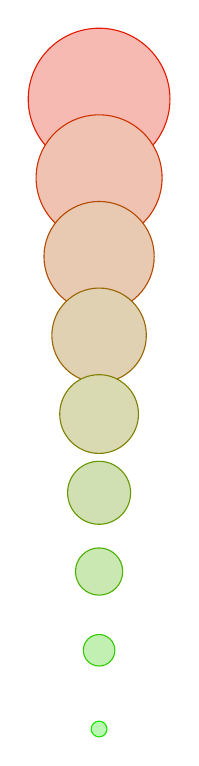
\begin{tikzpicture}
        \draw [red!90!green, fill=.!30!white] (0, 9) circle [radius=0.9];
        \draw [red!80!green, fill=.!30!white] (0, 8) circle [radius=0.8];
        \draw [red!70!green, fill=.!30!white] (0, 7) circle [radius=0.7];
        \draw [red!60!green, fill=.!30!white] (0, 6) circle [radius=0.6];
        \draw [red!50!green, fill=.!30!white] (0, 5) circle [radius=0.5];
        \draw [red!40!green, fill=.!30!white] (0, 4) circle [radius=0.4];
        \draw [red!30!green, fill=.!30!white] (0, 3) circle [radius=0.3];
        \draw [red!20!green, fill=.!30!white] (0, 2) circle [radius=0.2];
        \draw [red!10!green, fill=.!30!white] (0, 1) circle [radius=0.1];
    \end{tikzpicture}
\end{document}

